% This file was created by matlab2tikz.
%
%The latest updates can be retrieved from
%  http://www.mathworks.com/matlabcentral/fileexchange/22022-matlab2tikz-matlab2tikz
%where you can also make suggestions and rate matlab2tikz.
%
\definecolor{mycolor1}{rgb}{0.20810,0.16630,0.52920}%
\definecolor{mycolor2}{rgb}{0.02650,0.61370,0.81350}%
\definecolor{mycolor3}{rgb}{0.64730,0.74560,0.41880}%
\definecolor{mycolor4}{rgb}{0.97630,0.98310,0.05380}%
%
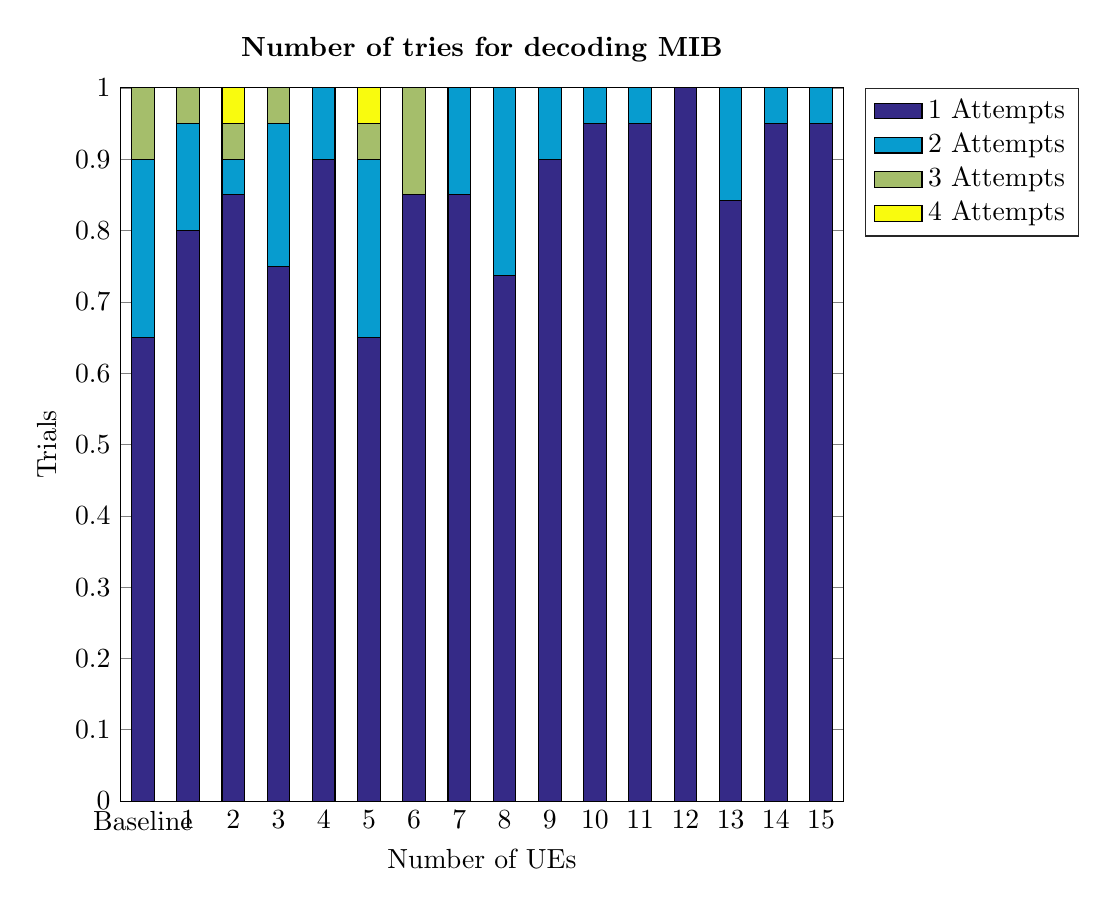
\begin{tikzpicture}

\begin{axis}[%
width=3.617in,
height=3.566in,
at={(0.607in,0.481in)},
scale only axis,
bar width=0.5,
xmin=-0.5,
xmax=15.5,
xtick={0,1,2,3,4,5,6,7,8,9,10,11,12,13,14,15},
xticklabels={{Baseline},{1},{2},{3},{4},{5},{6},{7},{8},{9},{10},{11},{12},{13},{14},{15}},
xlabel={Number of UEs},
ymin=0,
ymax=1,
ylabel={Trials},
axis background/.style={fill=white},
title style={font=\bfseries},
title={Number of tries for decoding MIB},
legend style={at={(1.03,1)},anchor=north west,legend cell align=left,align=left,draw=white!15!black}
]
\addplot[ybar stacked,draw=black,fill=mycolor1,area legend] plot table[row sep=crcr] {%
0	0.65\\
1	0.8\\
2	0.85\\
3	0.75\\
4	0.9\\
5	0.65\\
6	0.85\\
7	0.85\\
8	0.736842105263158\\
9	0.9\\
10	0.95\\
11	0.95\\
12	1\\
13	0.842105263157895\\
14	0.95\\
15	0.95\\
};
\addlegendentry{1 Attempts};

\addplot[ybar stacked,draw=black,fill=mycolor2,area legend] plot table[row sep=crcr] {%
0	0.25\\
1	0.15\\
2	0.05\\
3	0.2\\
4	0.1\\
5	0.25\\
6	0\\
7	0.15\\
8	0.263157894736842\\
9	0.1\\
10	0.05\\
11	0.05\\
12	0\\
13	0.157894736842105\\
14	0.05\\
15	0.05\\
};
\addlegendentry{2 Attempts};

\addplot[ybar stacked,draw=black,fill=mycolor3,area legend] plot table[row sep=crcr] {%
0	0.1\\
1	0.05\\
2	0.05\\
3	0.05\\
4	0\\
5	0.05\\
6	0.15\\
7	0\\
8	0\\
9	0\\
10	0\\
11	0\\
12	0\\
13	0\\
14	0\\
15	0\\
};
\addlegendentry{3 Attempts};

\addplot[ybar stacked,draw=black,fill=mycolor4,area legend] plot table[row sep=crcr] {%
0	0\\
1	0\\
2	0.05\\
3	0\\
4	0\\
5	0.05\\
6	0\\
7	0\\
8	0\\
9	0\\
10	0\\
11	0\\
12	0\\
13	0\\
14	0\\
15	0\\
};
\addlegendentry{4 Attempts};

\end{axis}
\end{tikzpicture}%